\chapter{Présentation de l'application}
\label{chap:realisation}

Ce chapitre présente l'interface de l'application telle qu'elle se comporte réellement, à travers les principaux écrans utilisés par un agent, par un validateur et par le personnel des ressources humaines. Chaque capture correspond à un usage effectif de l'application en environnement de développement, avec des comptes de démonstration représentant les différents rôles du circuit hiérarchique.

\section{Authentification}

L'accès à l'application se fait par matricule et mot de passe, conformément au besoin exprimé par le ministère. Un agent nouvellement créé reçoit un mot de passe temporaire qu'il doit obligatoirement changer à sa première connexion.

\begin{figure}[htbp]
    \centering
    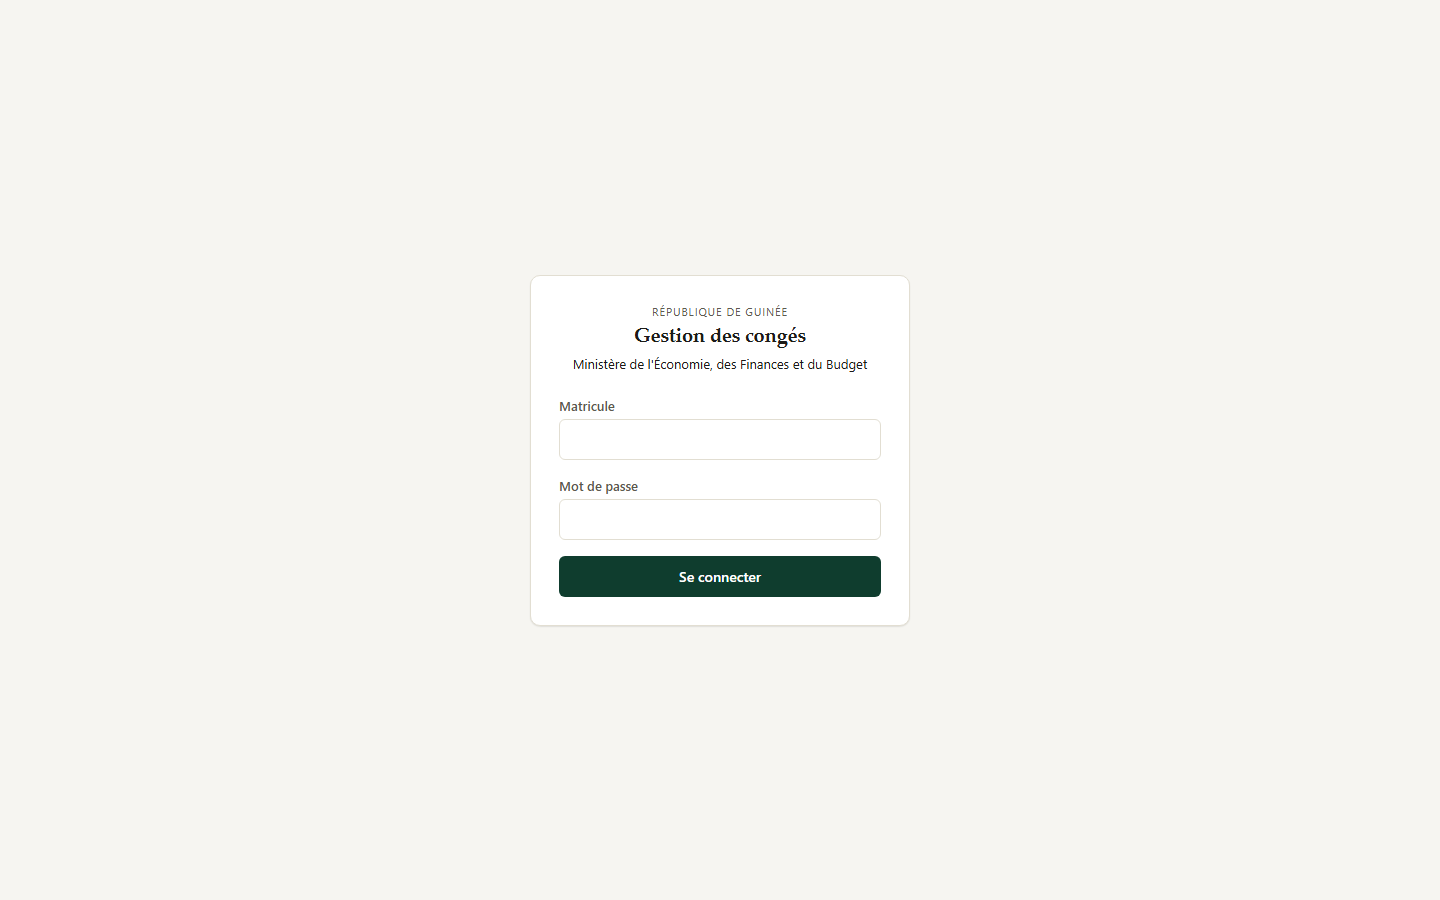
\includegraphics[width=0.55\textwidth]{images/01-connexion.png}
    \caption{Écran de connexion}
    \label{fig:connexion}
\end{figure}

\clearpage
\section{Dépôt d'une demande de congé}

Un agent commence par choisir un type de congé. Le formulaire affiche alors immédiatement la durée attendue et la liste des justificatifs requis pour ce type précis, sans que l'agent ait besoin de les connaître à l'avance.

\begin{figure}[htbp]
    \centering
    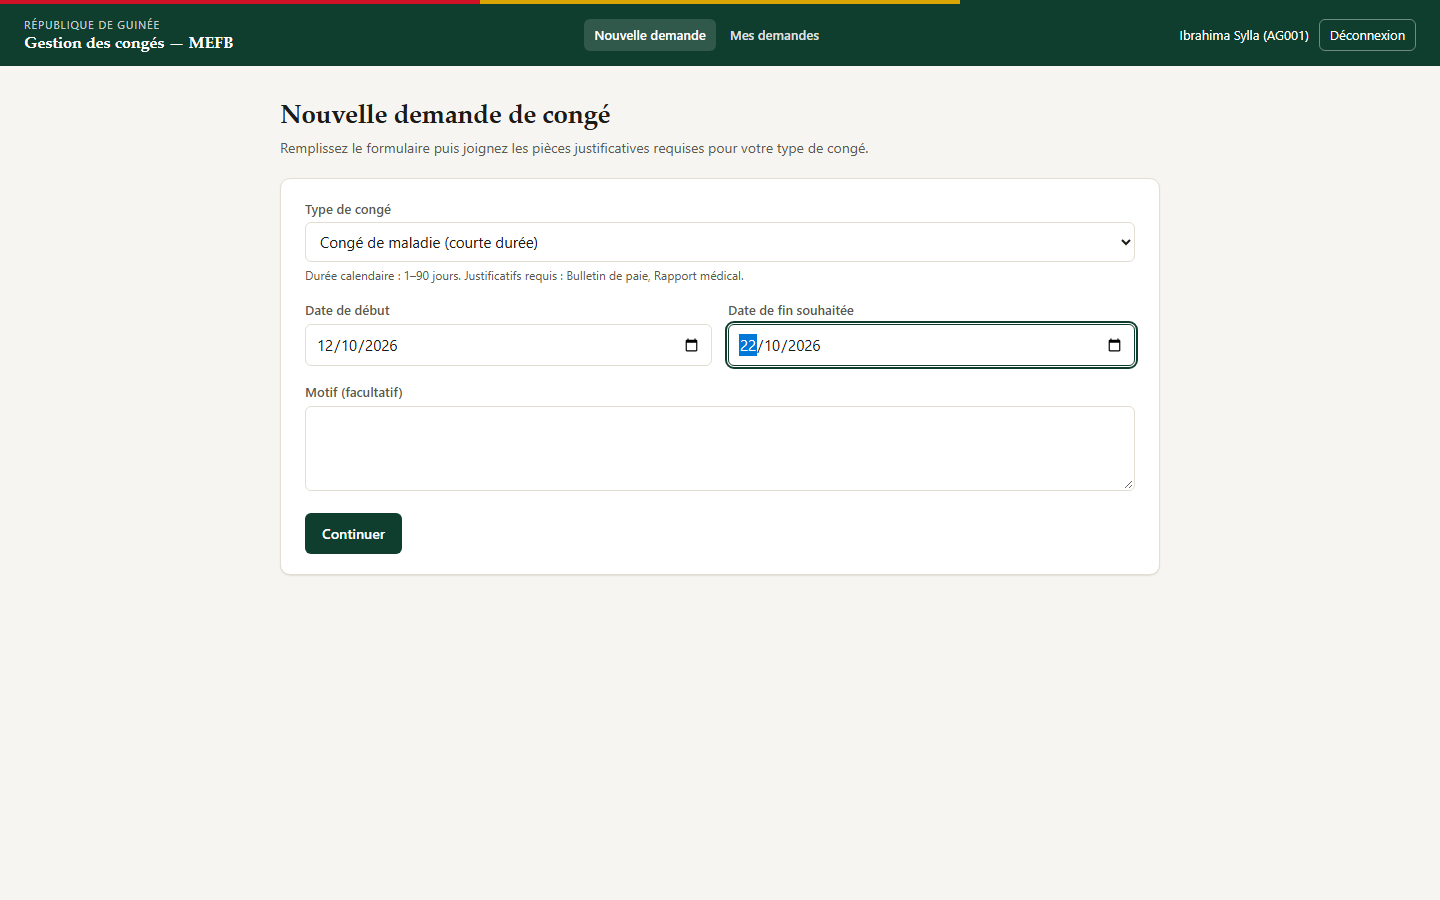
\includegraphics[width=\textwidth]{images/02-nouvelle-demande.png}
    \caption{Formulaire de nouvelle demande, avec les règles du type de congé sélectionné}
    \label{fig:nouvelle-demande}
\end{figure}

Une fois les informations saisies, l'agent est invité à joindre les pièces justificatives correspondantes avant de pouvoir soumettre sa demande. Le bouton de soumission reste désactivé tant qu'un justificatif obligatoire manque.

\begin{figure}[htbp]
    \centering
    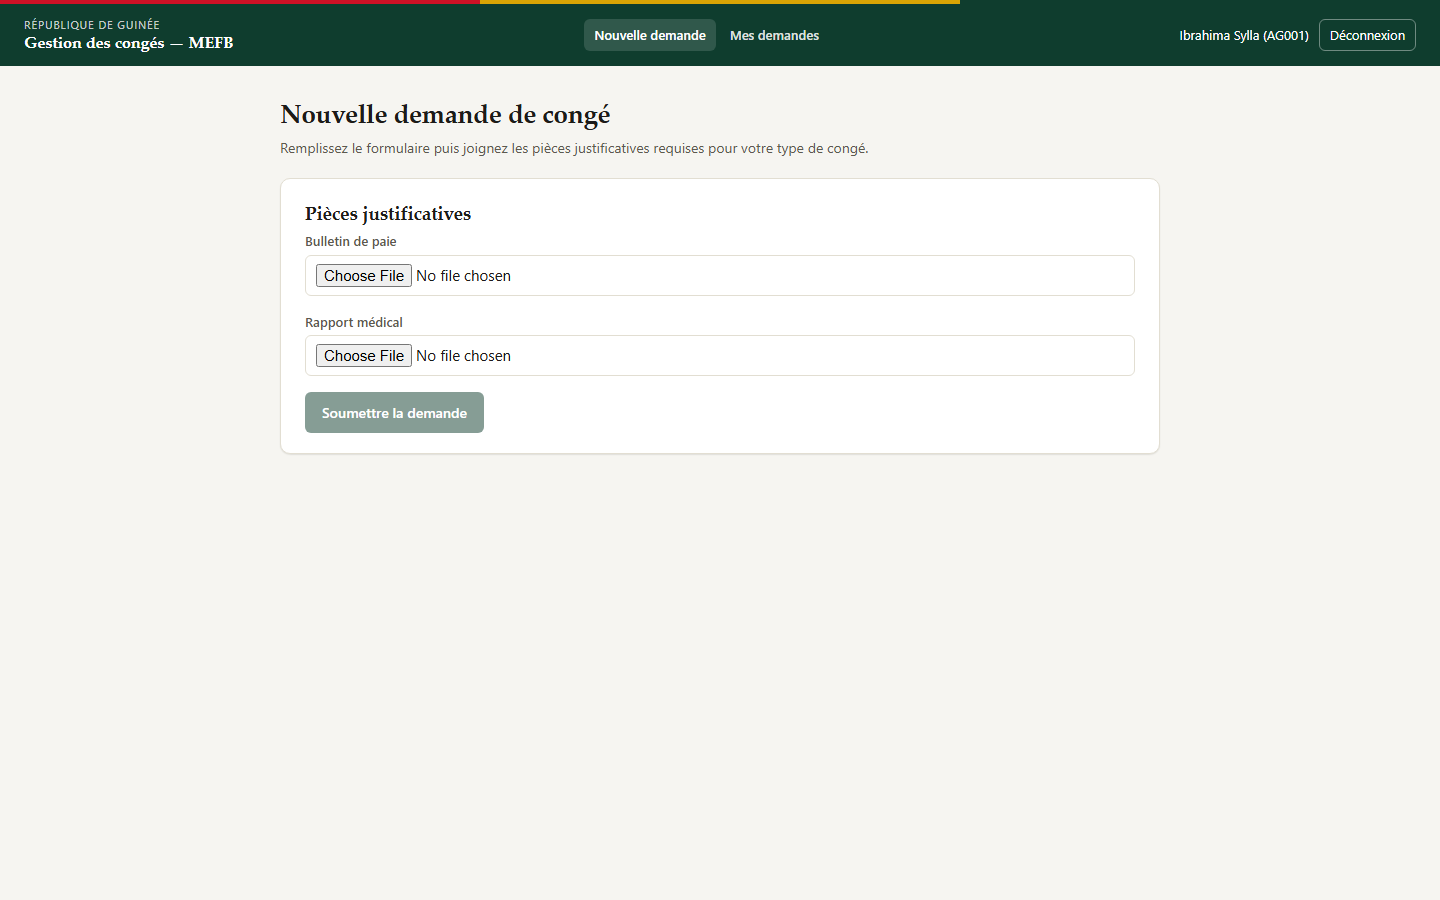
\includegraphics[width=\textwidth]{images/03-justificatifs.png}
    \caption{Dépôt des pièces justificatives requises}
    \label{fig:justificatifs}
\end{figure}

\clearpage
\section{Suivi des demandes}

L'agent retrouve l'historique de ses demandes, avec leur statut à jour, dans un tableau synthétique.

\begin{figure}[htbp]
    \centering
    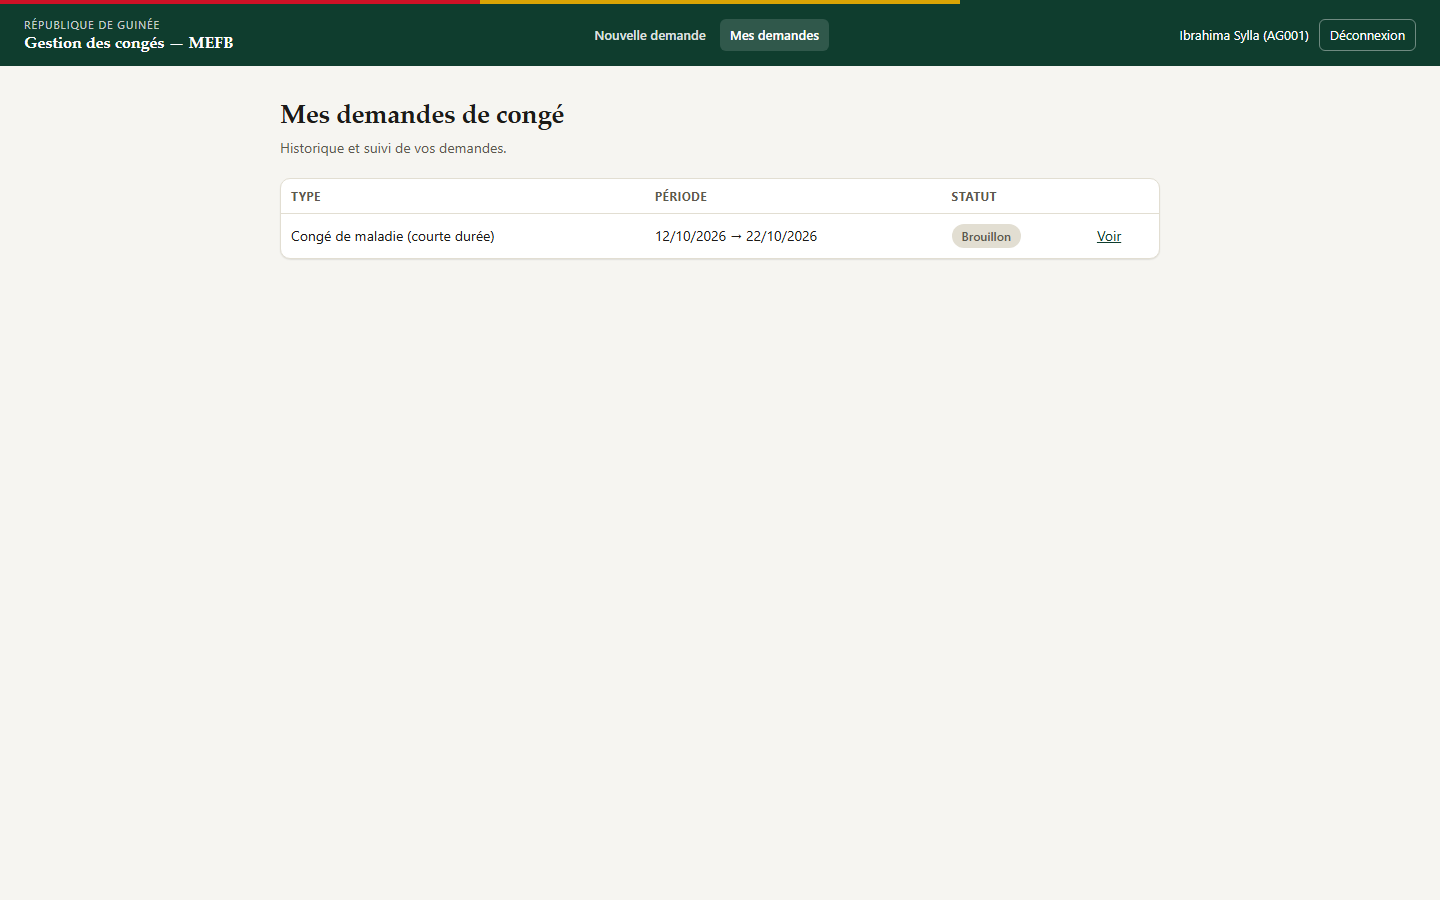
\includegraphics[width=\textwidth]{images/04-mes-demandes.png}
    \caption{Liste des demandes d'un agent}
    \label{fig:mes-demandes}
\end{figure}

En ouvrant une demande, l'agent visualise le détail du circuit de validation en cours, étape par étape, avec le nom du validateur attendu à chaque niveau. Tant qu'aucune décision définitive n'a été prise, il peut également annuler sa demande.

\begin{figure}[htbp]
    \centering
    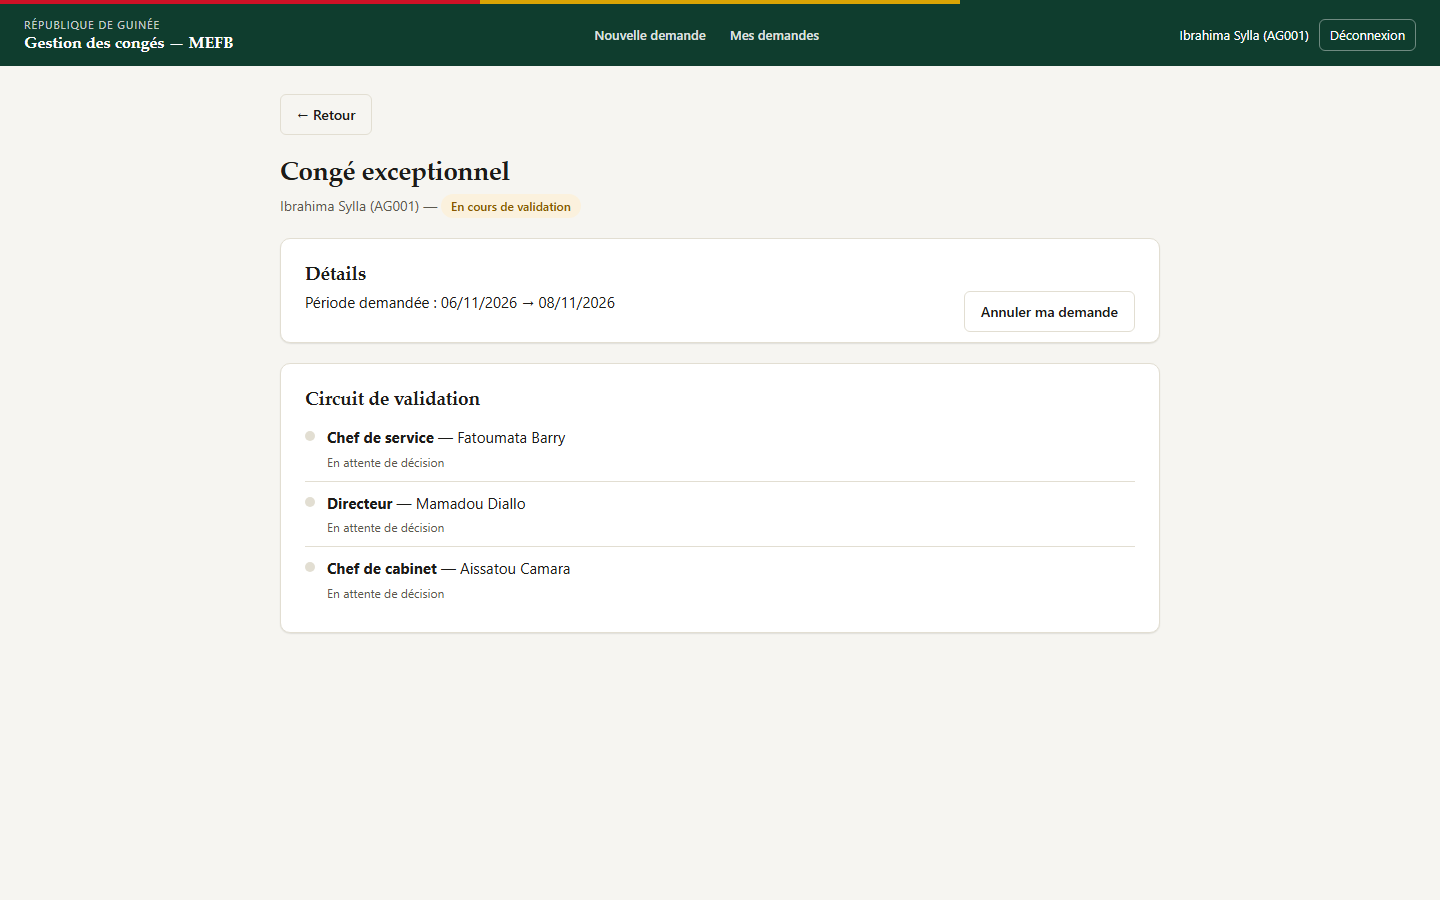
\includegraphics[width=\textwidth]{images/05-detail-demande-en-cours.png}
    \caption{Détail d'une demande en cours de validation}
    \label{fig:detail-demande}
\end{figure}

\clearpage
\section{Validation hiérarchique}

Chaque validateur (chef de service, directeur ou chef de cabinet) dispose d'une file d'attente listant uniquement les demandes qui requièrent effectivement sa décision à l'instant présent.

\begin{figure}[htbp]
    \centering
    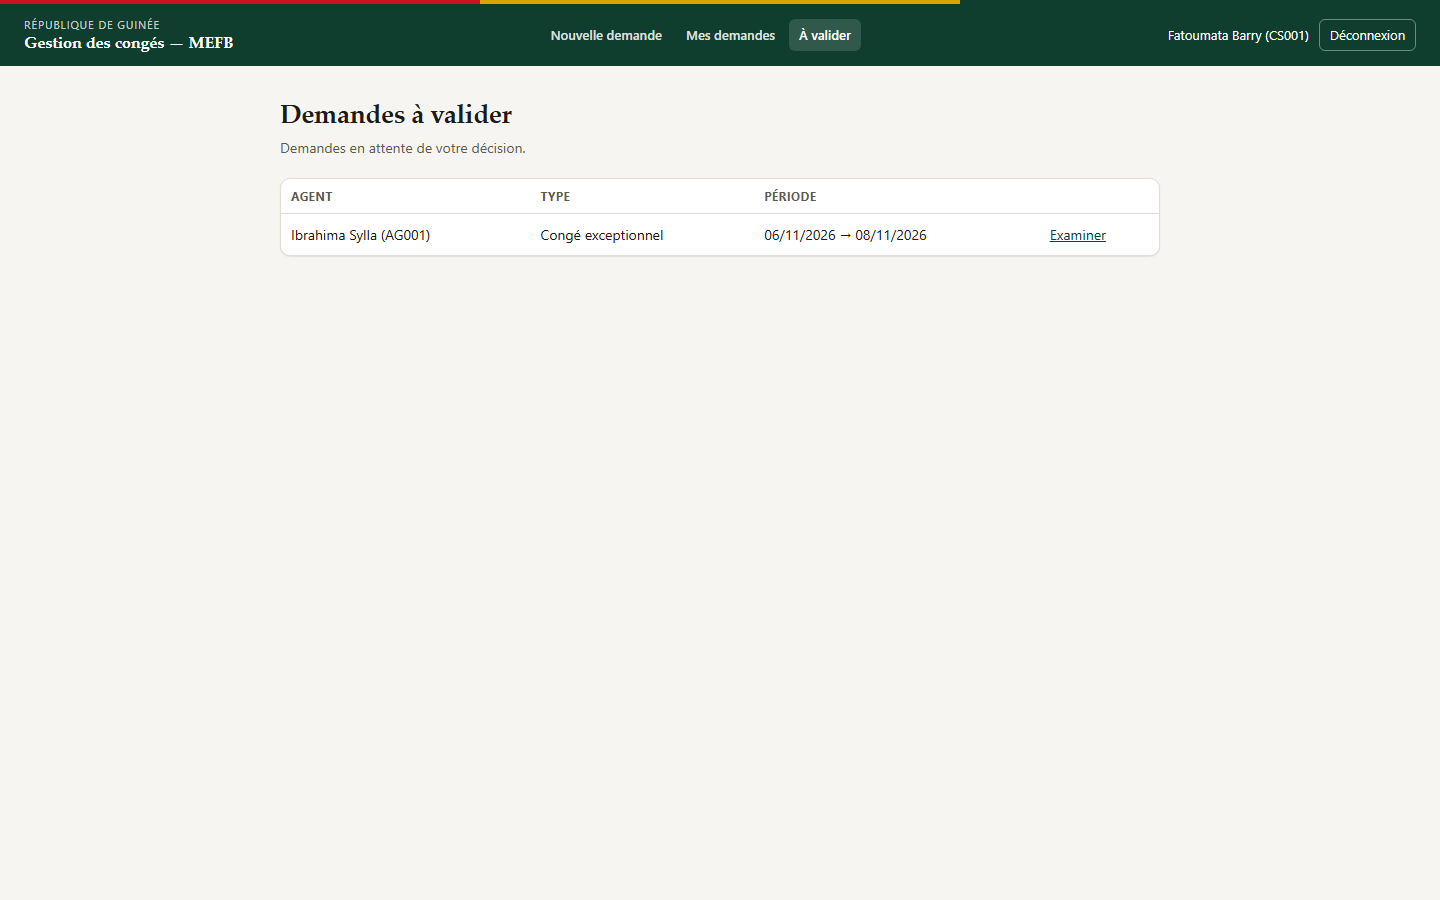
\includegraphics[width=\textwidth]{images/06-a-valider.png}
    \caption{File des demandes à valider}
    \label{fig:a-valider}
\end{figure}

En ouvrant une demande depuis cette file, le validateur retrouve le même circuit que l'agent, complété d'un panneau lui permettant d'approuver ou de rejeter la demande, avec un commentaire obligatoire en cas de rejet.

\begin{figure}[htbp]
    \centering
    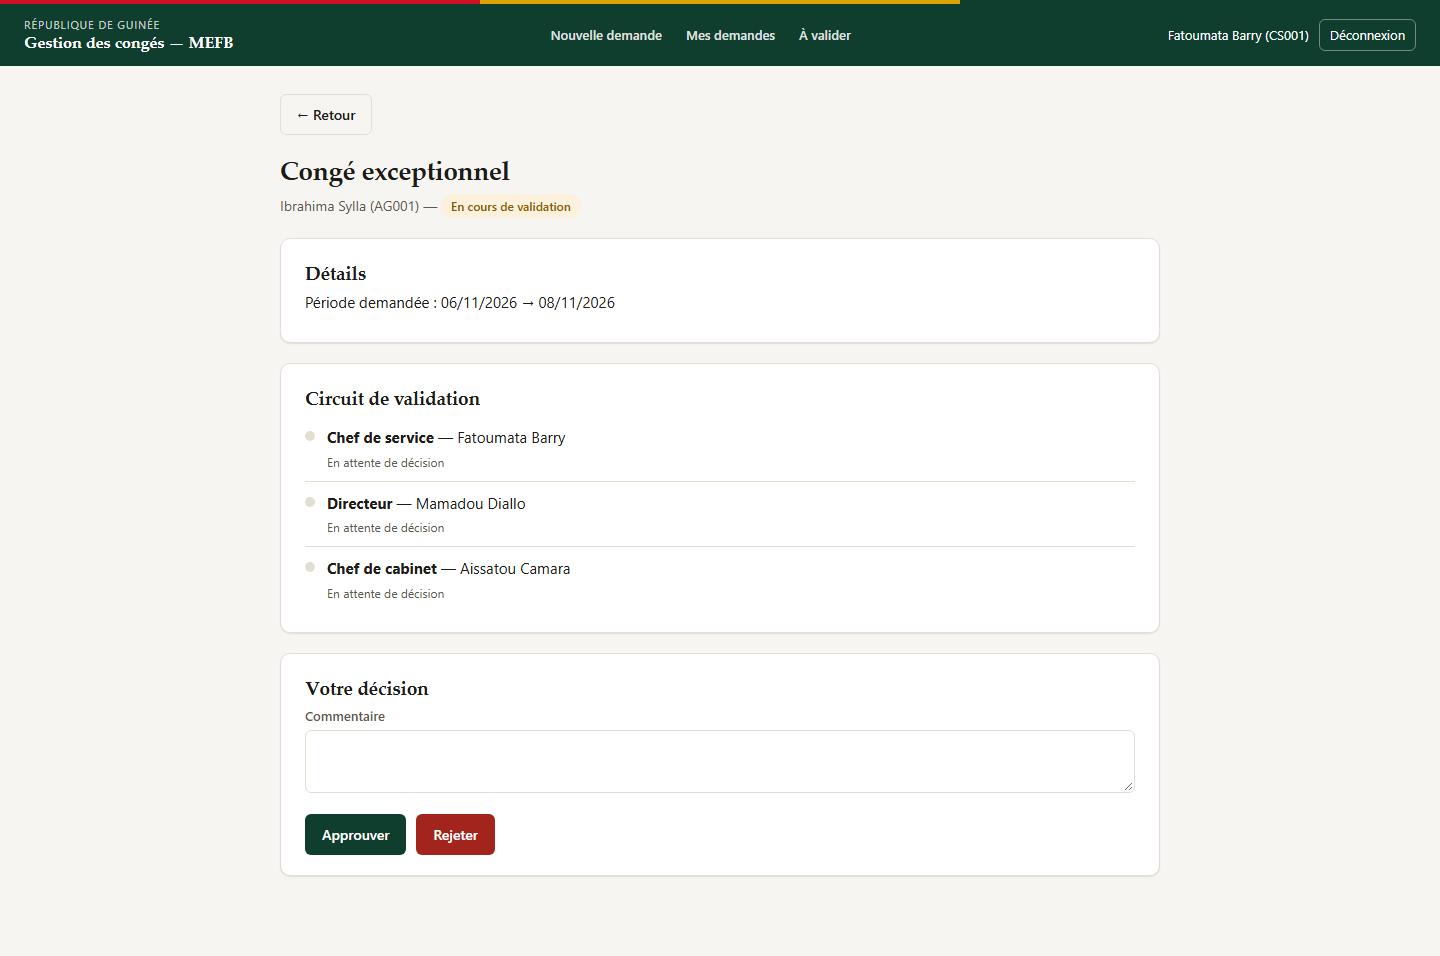
\includegraphics[width=\textwidth]{images/07-decision-validation.png}
    \caption{Prise de décision par un validateur}
    \label{fig:decision-validation}
\end{figure}

\clearpage
\section{Attestation}

Lorsque la dernière étape du circuit est approuvée, l'application génère automatiquement une attestation, immédiatement consultable depuis la demande concernée. Le numéro de série qui y figure permet d'en vérifier l'authenticité de manière indépendante, sans avoir à se connecter à l'application.

\begin{figure}[htbp]
    \centering
    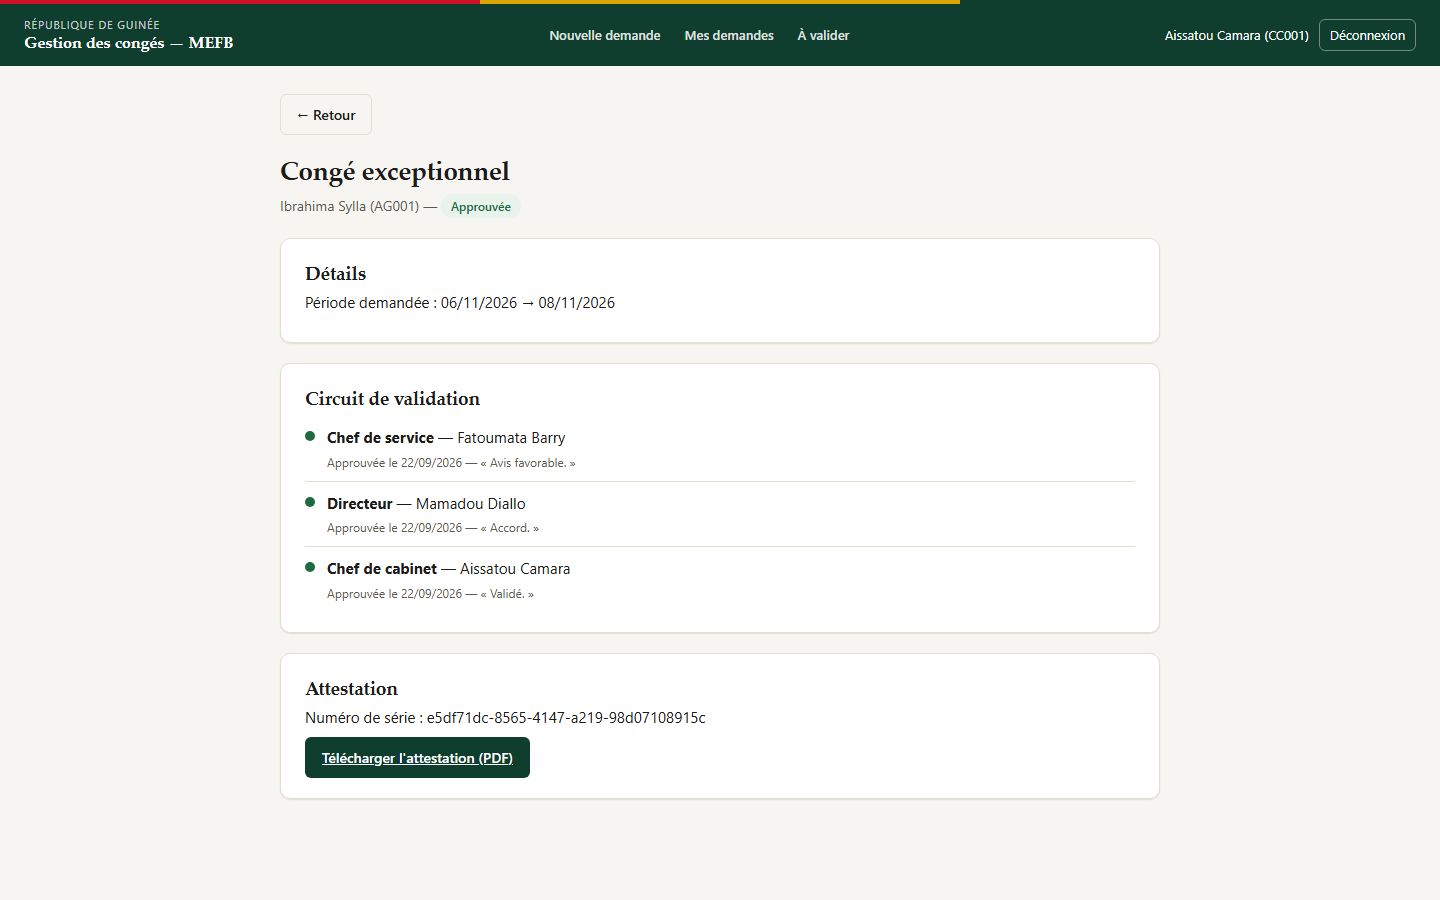
\includegraphics[width=\textwidth]{images/08-attestation-generee.png}
    \caption{Demande approuvée et attestation disponible}
    \label{fig:attestation}
\end{figure}

\clearpage
\section{Administration des comptes et de l'organisation}

Le personnel des ressources humaines dispose d'écrans dédiés pour créer les comptes des agents et gérer la structure organisationnelle du ministère, dont dépend directement le calcul du circuit de validation de chaque demande.

\begin{figure}[htbp]
    \centering
    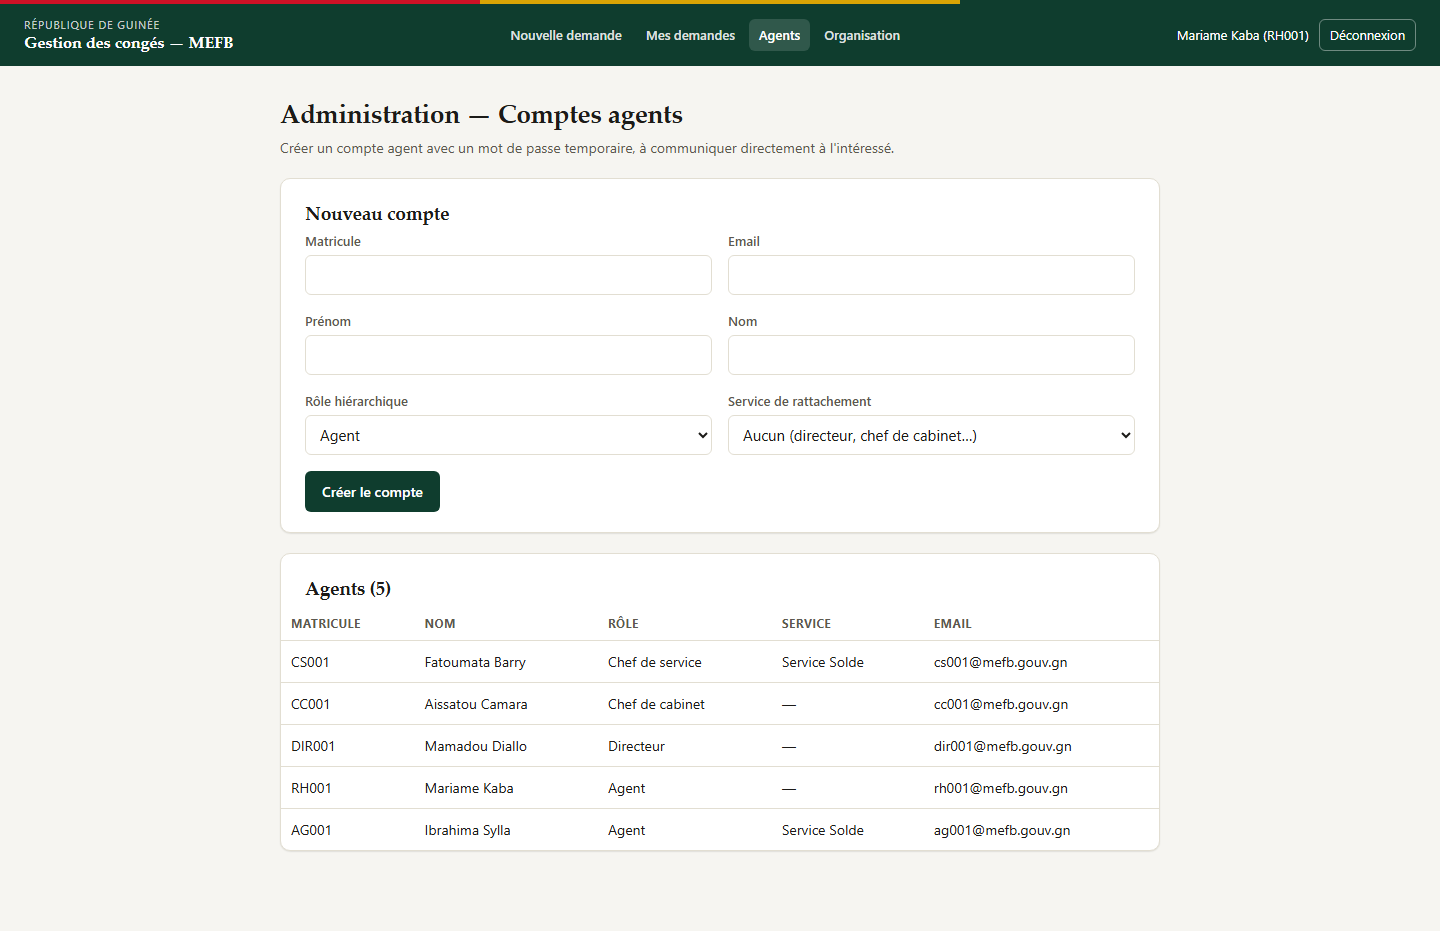
\includegraphics[width=\textwidth]{images/09-administration-agents.png}
    \caption{Création et consultation des comptes agents}
    \label{fig:administration-agents}
\end{figure}

\begin{figure}[htbp]
    \centering
    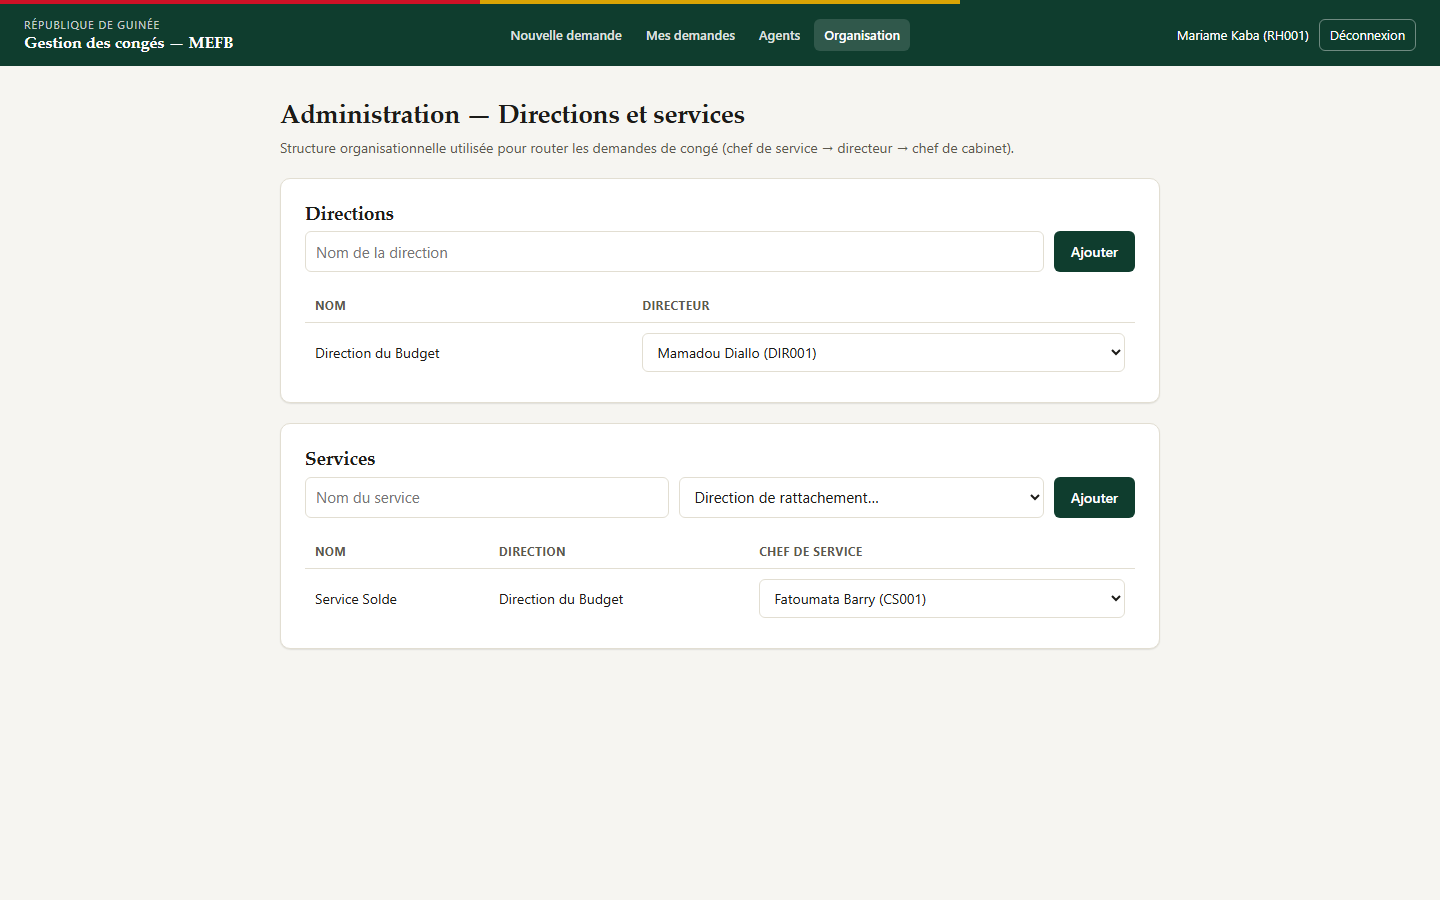
\includegraphics[width=\textwidth]{images/10-administration-organisation.png}
    \caption{Gestion des directions et des services}
    \label{fig:administration-organisation}
\end{figure}
